\section{Техническое задание}
\subsection{Основание для разработки}

Полное наименование системы: "<Интернет-магазин декоративных растений">.

Основанием для разработки программы является приказ ректора ЮЗГУ от <<04>> апреля 2024 г. №1616-с <<Об утверждении тем выпускных квалификационных работ>>.


\subsection{Цель и назначение разработки}

Программно-информационная система предназначена для продажи растений через Интернет.
С системой должны работать следующие группы пользователей:
\begin{itemize}
	\item администратор интернет-магазина;
	\item посетитель интернет-магазина.
\end{itemize}

Администратор должен иметь возможность добавлять, удалять и редактировать товары и свои категории. Например, "<акции"> или "<новинки">.
Посетитель интернет-магазина должен иметь возможность просматривать товары, добавлять их в корзину и оформлять заказ.

Задачами данной разработки являются:
\begin{itemize}
	\item проектирование базы данных;
	\item проектирование пользовательского интерфейса;
	\item разработка методов отображения данных из базы данных;
	\item разработка методов управления базой данных администратором.
\end{itemize}

\subsection{Требования к программной системе}

\subsubsection{Требования к данным}
Входными данными для системы являются:
\begin{itemize}
	\item информация о пользователе, предоставляемая им в процессе регистрации в системе;
	\item информация о пользователе, предоставляемая им в процессе оформления заказа;
	\item информация о товарных позициях (отдельных товарах) заказа;
	\item параметры фильтрации товаров;
	\item информация о товарах, вводимая администратором;
	\item информация о категориях, вводимая администратором.
\end{itemize}

Выходными данными для системы являются:
\begin{itemize}
	\item стоимость всех товаров в корзине;
	\item список заказов;
	\item уведомление о добавлении товара в корзину;
	\item уведомление об удалении товара из корзины;
	\item уведомление об оформленном заказе;
	\item сообщения об ошибках;
	\item ссылки для переадресации (URL).
\end{itemize}


\subsubsection{Функциональные требования}

Сайт имеет две группы пользователей с разными правами: администраторы и покупатели.

На рисунке ~\ref{admin:image} изображены прецеденты для администратора сайта.

\begin{figure}[h!]
	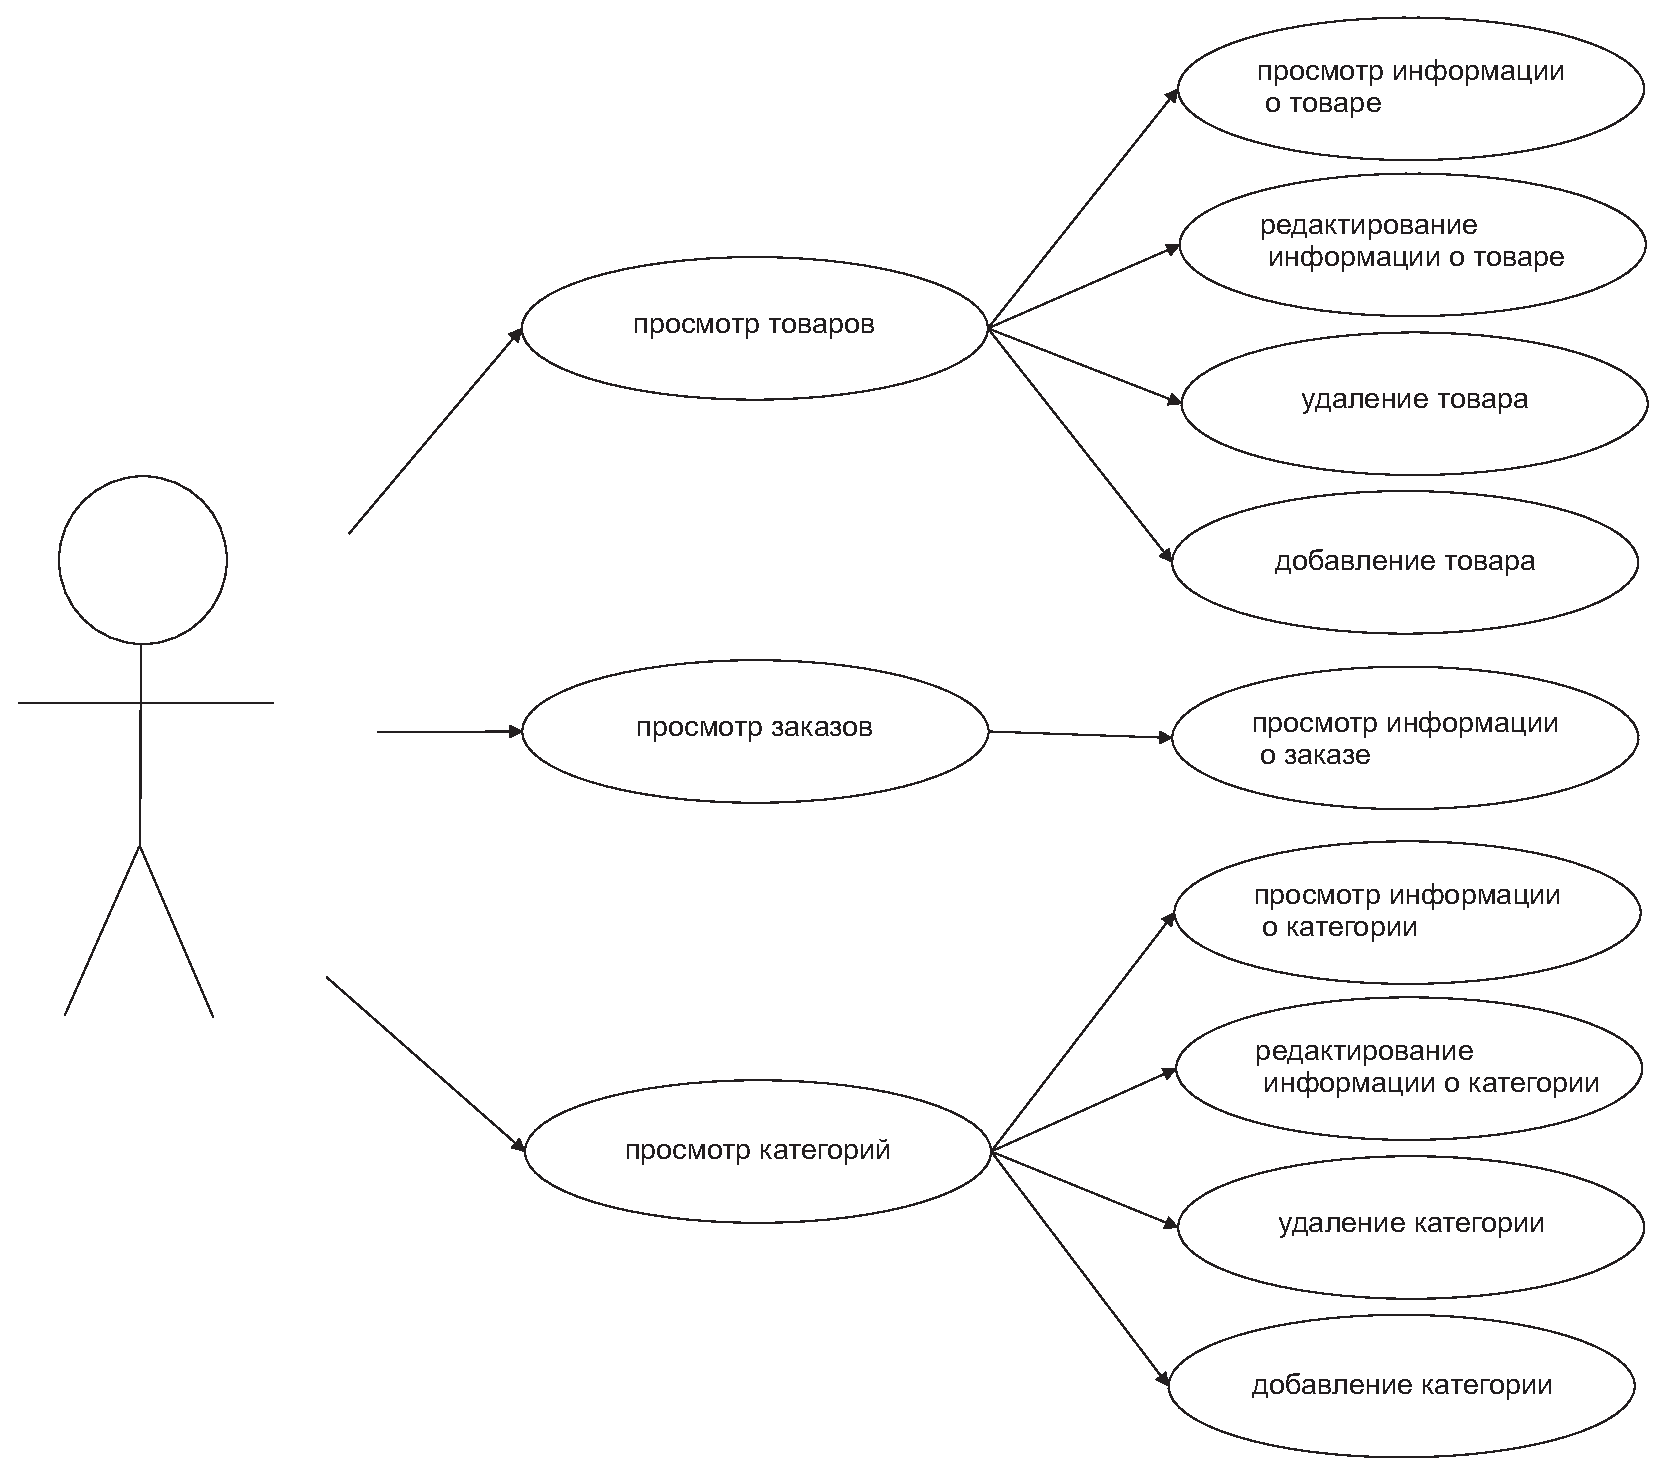
\includegraphics[width=0.8\linewidth]{admin}
	\caption{Прецеденты для администратора}
	\label{admin:image}
\end{figure}
%\vspace{-\figureaboveskip} % двойной отступ не нужен (можно использовать, если раздел заканчивается картинкой)

На рисунке ~\ref{user:image} изображены прецеденты для покупателя.
\begin{figure}[h!]
	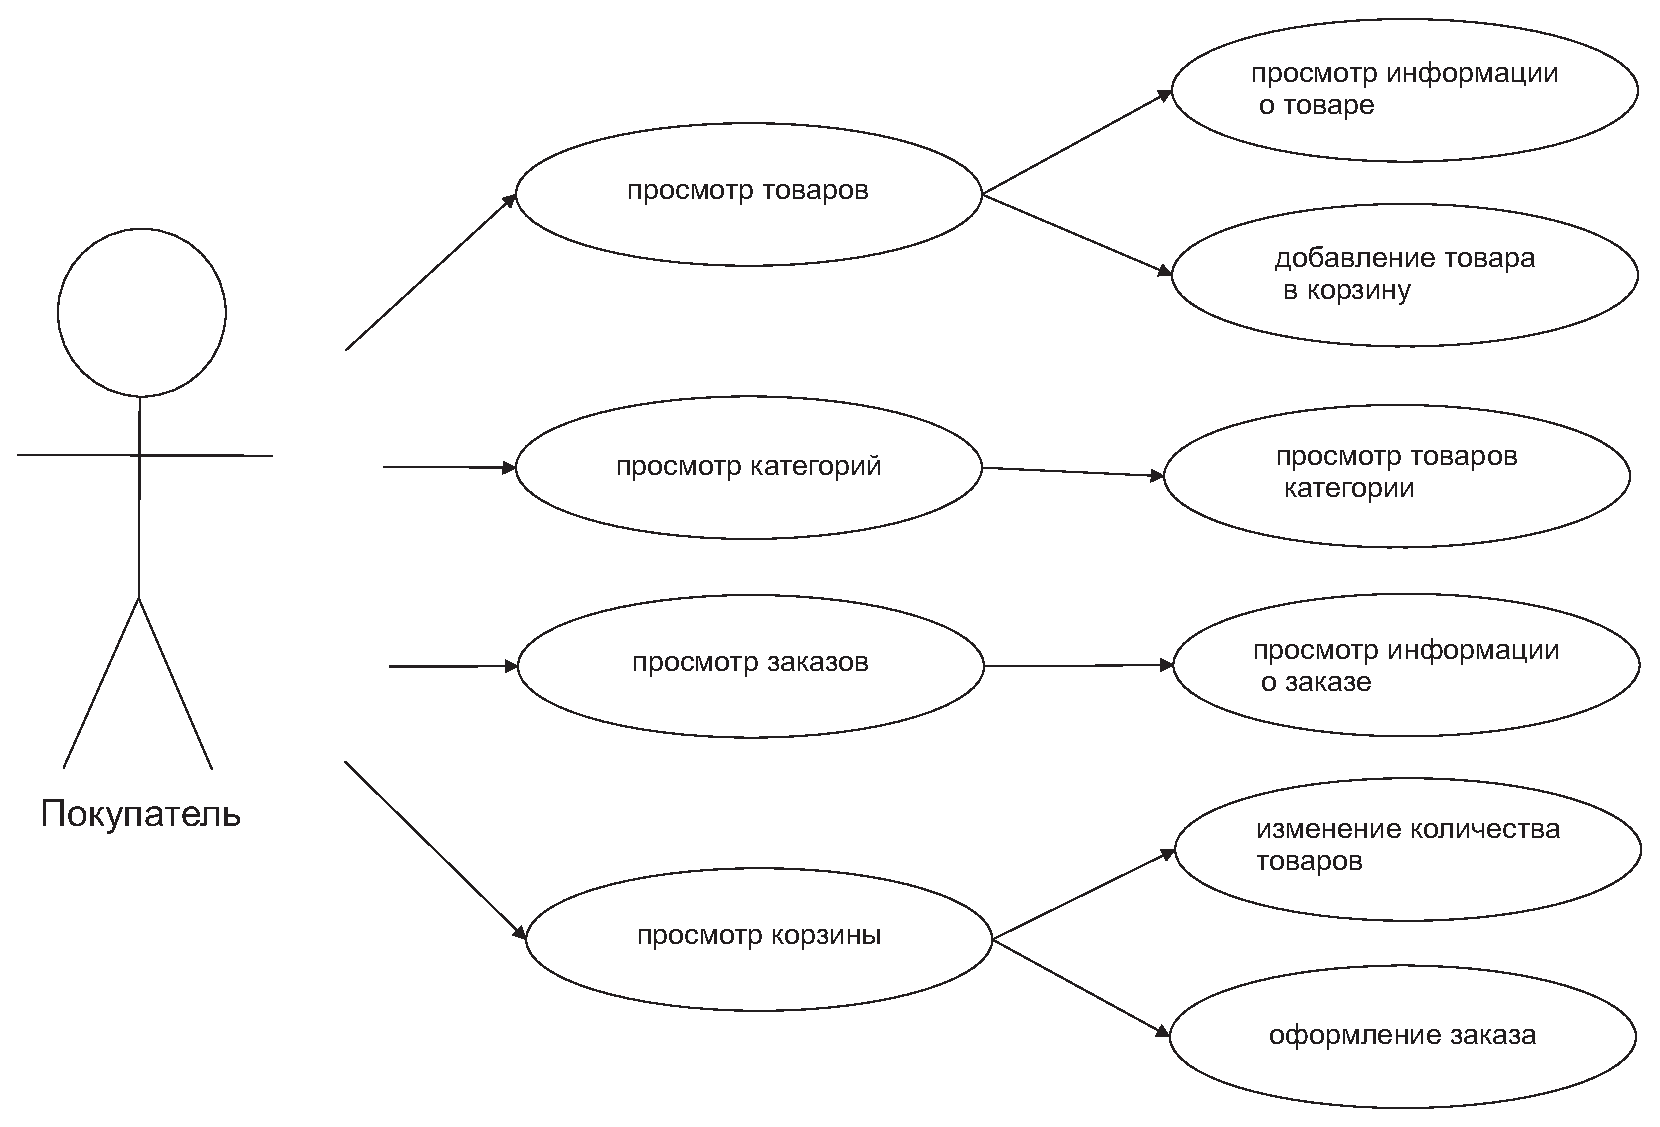
\includegraphics[width=0.8\linewidth]{user}
	\caption{Прецеденты для покупателя}
	\label{user:image}
\end{figure}
%\vspace{-\figureaboveskip} % двойной отступ не нужен (можно использовать, если раздел заканчивается картинкой)


\paragraph{Сценарий прецедента администратора «Просмотр информации о товаре»}

Основной успешный сценарий для прецедента «Просмотр информации о товаре»:
\begin{enumerate}
	\item Открыть страницу товаров.
	\item Нажать на кнопку «Открыть» рядом с товаром, о котором нужно узнать информацию.
	\item Ознакомиться с представленной информацией.
\end{enumerate}

\paragraph{Сценарий прецедента администратора «Редактирование информации о товаре»}

Основной успешный сценарий для прецедента «Редактирование информации о товаре»:
\begin{enumerate}
	\item Открыть страницу товаров.
	\item Нажать на кнопку «Изменить» рядом с товаром, информацию о котором нужно отредактировать.
	\item Переписать информацию в некоторых полях.
	\item Нажать на кнопку «Редактировать».
\end{enumerate}

\paragraph{Сценарий прецедента администратора «Удаление товара»}

Основной успешный сценарий для прецедента «Удаление товара»:
\begin{enumerate}
	\item Открыть страницу товаров.
	\item Нажать на кнопку Удалить» рядом с нужным товаром.
\end{enumerate}

\paragraph{Сценарий прецедента администратора «Добавление товара»}

Основной успешный сценарий для прецедента «Добавление товара»:
\begin{enumerate}
	\item Открыть страницу товаров.
	\item Нажать на кнопку «Добавить» в нижней части страницы.
	\item Написать информацию о товаре.
	\item Нажать на кнопку «Готово».
\end{enumerate}

\paragraph{Сценарий прецедента администратора «Просмотр информации о заказе»}

Основной успешный сценарий для прецедента «Просмотр информации о заказе»:
\begin{enumerate}
	\item Открыть страницу заказов.
	\item Нажать на кнопку «Открыть» рядом с нужным заказом.
	\item Ознакомиться с представленной информацией.
\end{enumerate}

\paragraph{Сценарий прецедента администратора «Просмотр информации о категории»}

Основной успешный сценарий для прецедента «Просмотр информации о категории»:
\begin{enumerate}
	\item Открыть страницу категорий.
	\item Нажать на кнопку «Открыть» рядом с категорией, о которой нужно узнать информацию.
	\item Ознакомиться с представленной информацией.
\end{enumerate}

\paragraph{Сценарий прецедента администратора «Редактирование информации о категории»}

Основной успешный сценарий для прецедента «Редактирование информации о категории»:
\begin{enumerate}
	\item Открыть страницу категорий.
	\item Нажать на кнопку «Изменить» рядом с категорией, информацию о которой нужно Отредактировать.
	\item Переписать информацию в некоторых полях.
	\item Нажать на кнопку «Редактировать».
\end{enumerate}

\paragraph{Сценарий прецедента администратора «Удаление категории»}

Основной успешный сценарий для прецедента «Удаление категории»:
\begin{enumerate}
	\item Открыть страницу категорий.
	\item Нажать на кнопку Удалить» рядом с нужной категорией.
\end{enumerate}

\paragraph{Сценарий прецедента администратора «Добавление категории»}

Основной успешный сценарий для прецедента «Добавление категории»:
\begin{enumerate}
	\item Открыть страницу категорий.
	\item Нажать на кнопку «Добавить» в нижней части страницы.
	\item Написать информацию о категории.
	\item Нажать на кнопку «Готово».
\end{enumerate}


\paragraph{Сценарий прецедента покупателя «Просмотр информации о товаре»}
Предусловие: открыта страница всех товаров или товаров категории.

Основной успешный сценарий для прецедента «Просмотр информации о товаре»:
\begin{enumerate}
	\item Нажать на кнопку «Подробнее» в карточке интересующего товара.
	\item Ознакомиться с представленной информацией.
\end{enumerate}

\paragraph{Сценарий прецедента покупателя «Добавление товара в корзину»}
Предусловие: открыта страница всех товаров или товаров категории.

Основной успешный сценарий для прецедента «Добавление товара в корзину»:
\begin{enumerate}
	\item Нажать на кнопку «Подробнее» в карточке интересующего товара.
	\item Ознакомиться с представленной информацией.
	\item Нажать на кнопку «Добавить в корзину».
\end{enumerate}

\paragraph{Сценарий прецедента покупателя «Просмотр товаров категории»}

Основной успешный сценарий для прецедента «Просмотр товаров категории»:
\begin{enumerate}
	\item Открыть страницу «Категории».
	\item Нажать на интересующую категорию.
	\item Ознакомиться с представленными товарами.
\end{enumerate}

\paragraph{Сценарий прецедента покупателя «Просмотр информации о заказе»}
Предусловие: наличие заказов.

Основной успешный сценарий для прецедента «Просмотр информации о заказе»:
\begin{enumerate}
	\item Открыть страницу заказов.
	\item Нажать на кнопку «Открыть» рядом с нужным заказом.
	\item Ознакомиться с представленной информацией.
\end{enumerate}

\paragraph{Сценарий прецедента покупателя «Изменение количества товара»}
Предусловие: наличие товаров в корзине.

Основной успешный сценарий для прецедента «Изменение количества товара»:
\begin{enumerate}
	\item Открыть корзину.
	\item Нажимать на кнопку увеличения или уменьшения количества около нужного товара, пока не получится требуемое число.
\end{enumerate}

\paragraph{Сценарий прецедента покупателя «Оформление заказа»}
Предусловие: наличие товаров в корзине.

Основной успешный сценарий для прецедента «Оформление заказа»:
\begin{enumerate}
	\item Открыть корзину.
	\item Нажать на кнопку «Оформить заказ».
	\item Ввести необходимую информацию.
	\item Нажать на кнопку «Оформить заказ».
\end{enumerate}

\subsubsection{Требования пользователя к интерфейсу web-сайта}

Сайт должен иметь следующие страницы:
\begin{itemize}
	\item главная страница со всеми товарами;
	\item страница категорий товаров;
	\item страница товаров, принадлежащих выбранной категории;
	\item корзина;
	\item список заказов.
\end{itemize}

Администратору также необходимы страницы для редактирования, удаления и добавления товаров и категорий.

Товары на главной странице должны быть представлены в виде карточек одинакового размера, содержащих фото, название и цену товара. Пользователь должен иметь возможность фильтровать растения по характеристикам.

Макет страницы с товарами приведён на рисунке ~\ref{interface:image}.

\begin{figure}[ht]
	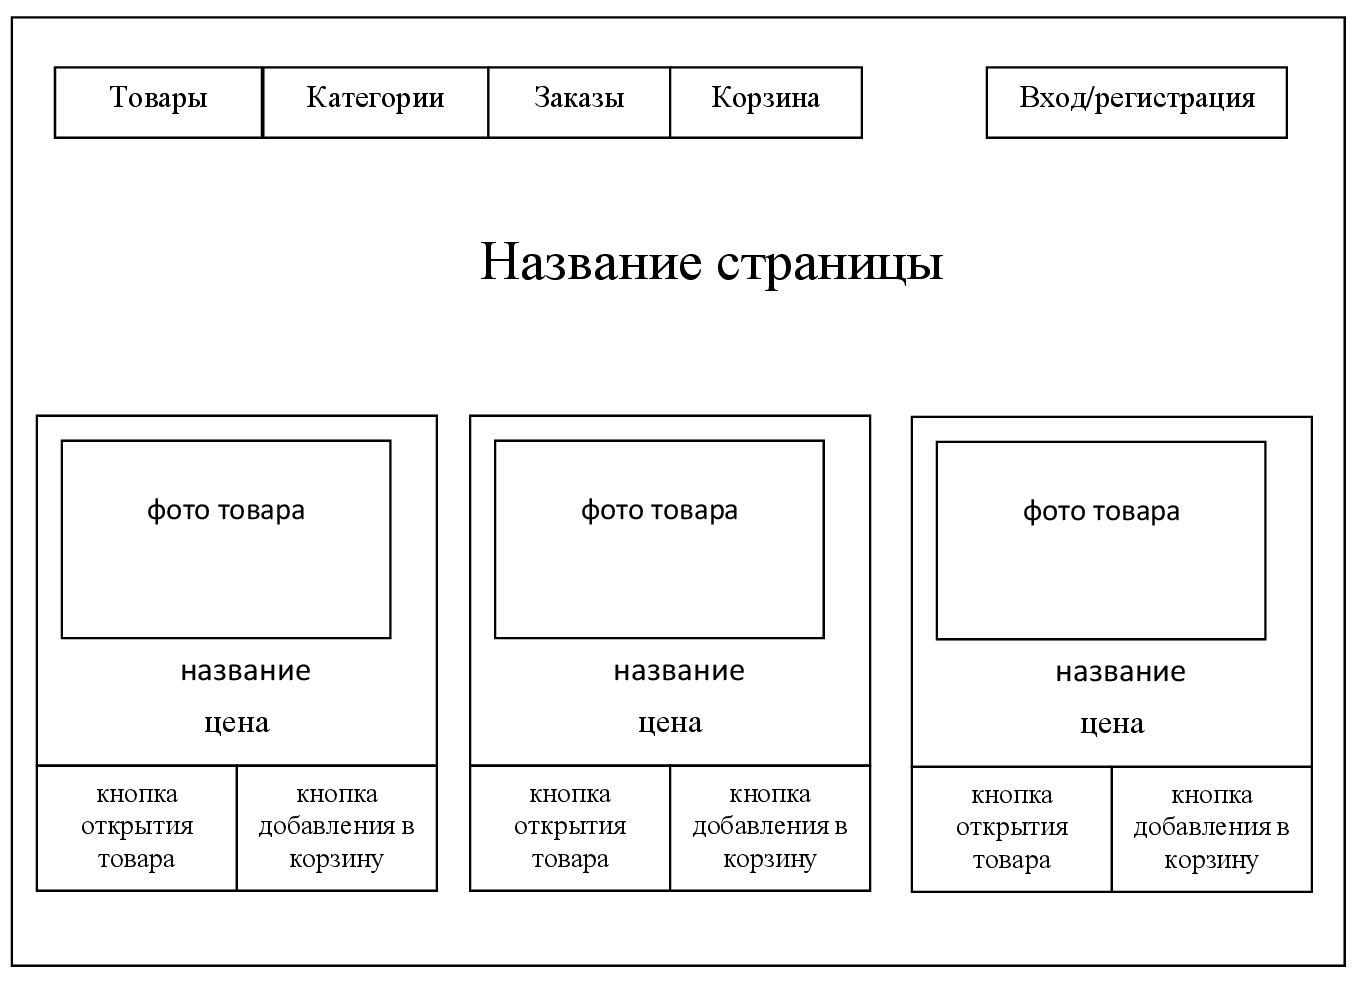
\includegraphics[width=1\linewidth]{interface}
	\caption{Макет страницы с товарами}
	\label{interface:image}
\end{figure}
%\vspace{-\figureaboveskip} % двойной отступ не нужен (можно использовать, если раздел заканчивается картинкой)

\subsubsection{Нефункциональные требования}

\paragraph{Требования к безопасности}
Необходимо устранить уязвимости, возможные для веб-приложений:
\begin{itemize}
	\item Межсайтовые скрипты (XSS) — это уязвимость системы безопасности, которая позволяет злоумышленнику размещать клиентские скрипты (обычно JavaScript) на веб-страницах. Когда другие пользователи загружают затронутые страницы, будут выполняться скрипты злоумышленника, что позволяет злоумышленнику украсть cookie-маркеры и маркеры сеанса, изменить содержимое веб-страницы с помощью DOM или перенаправить браузер на другую страницу.
	\item SQL-инъекция (Внедрение SQL-кода) — это попытка изменить запрос к базе данных. Ввести ее можно через форму или ссылку, которая передает параметры методом GET\cite{dronov}.
	\item Доступ обычного пользователя к возможностям администратора.
	\item Межсайтовая подделка запроса (CSRF) — это вид атак на сайт, при котором злоумышленник с помощью мошеннического сайта или скрипта заставляет браузер пользователя выполнять на доверенном сайте действия от его имени: отправлять сообщения, менять пароли, переводить деньги и пр. В атаке используются недостатки протокола HTTP. Чтобы стать жертвой, пользователю достаточно перейти по вредоносной ссылке.
\end{itemize}

\paragraph{Требования к программному обеспечению}
Для реализации программной системы необходимо подготовить следующие компоненты:
\begin{itemize}
	\item пакетный менеджер Composer для управления зависимостями;
	\item фреймворк Laravel;
	\item интерпретатор языка программирования PHP;
	\item СУБД MySQL;
	\item веб-сервер, поддерживающий PHP.
\end{itemize}

Laravel совместим со всеми современными операционными системами, включая Windows, macOS и Linux.

\paragraph{Требования к аппаратному обеспечению}
Для работы приложения требуется дисковое пространство не менее 2,5 Гб, минимум 2 Гб оперативной памяти и подключение к Интернету. Рекомендуется использовать процессор c 2 или более ядрами и частотой 2 ГГц или выше.

\subsection{Требования к оформлению документации}
Требования к стадиям разработки программ и программной документации для вычислительных машин, комплексов и систем независимо от их назначения и области применения, этапам и содержанию работ устанавливаются ГОСТ 19.102–77. 
Программная документация должна включать в себя: 
\begin{enumerate}
	\item Анализ предметной области.
	\item Техническое задание.
	\item Технический проект.
	\item Рабочий проект.
\end{enumerate}
